\chapter{Minería de Procesos}
\addcontentsline{toc}{chapter}{Minería de Procesos}

\section{Introducción a la minería de procesos}

Las transacciones de los agentes en estos mundos virtuales registradas en el servidor no sólo son importantes desde el punto de vista de la evaluación del alumnado, sino que también nos proporcionan información de cómo se han resuelto los problemas propuesto, hito por hito, y son un reflejo de la estrategia seguida por ccada uno de los equipos para intentar resolver todos los mundos.

Para tratar de desvelar estas estrategias ocultas se usarán técnicas de minería de procesos, considerando una estrategia como el proceso seguido por los estudiantes hasta llegar al objetivo. La minería de procesos puede definirse como la disciplina que tiene como objetivo descubrir, monitorear y mejorar procesos de negocio mediante el análisis de las transacciones del proceso que se han almacenado en algún sistema de información \citep{Mayorga_2015}.

Actualmente, con el desarrollo y el creciente interés de las plataformas educativas y de toda la tecnología relacionada con las mismas, los sistemas de información nos permiten recoger todo tipo de información. Esto puede incluir desde información de bajo nivel (clicks del ratón) hasta información de alto nivel (realización de una actividad en particular dentro de la plataforma). Es decir, estos sistemas tienen la capacidad de almacenar datos temporales de diversa índole, como cadenas de clicks, registros de chats, históricos de modificación de documentos, registros de uso de los diferentes recursos educativos, etc. \cite{Bogarin_2017}. La minería de procesos puede usar todos estos logs para descubrir, monitorear y mejorar los procesos educativos. Surge así la denominada minería de procesos educacional (en inglés, \emph{educational process mining}). No obstante, cabe destacar que, aunque en este trabajo fin de grado nos centraremos en la minería de procesos en el ámbito educativo, ésta también tiene númerosas aplicaciones en el área sanitaria, en el ámbito empresarial, institucional etc.

\section{Extracción de los procesos con DISCO}

Para la extracción de los procesos ocultos se empleará el programa Disco. Disco es una herramienta de minería de procesos profesional que permite crear mapas visuales a partir de los registros en cuestión de minutos.

Para crear los diagramas de Disco, se extraerán los campos de información más importantes del dataset:
\begin{enumerate}
\item El identificador del caso, extraído de una clave aleatoria generada al principio de cada operación \texttt{LOGIN} y que distingue de manera unívoca cada sesión de trabajo de los estudiantes.
\item El agente, que se refiere al nombre del grupo de estudiantes.
\item La fecha y hora a la que se registró la transacción.
\item El campo actividad (\texttt{Activity}), que refleja la acción de los alumnos en el mundo virtual.
\item Varios campos de tipo recurso (\texttt{Resource}) que proporcionan información adicional que puede sernos de utilidad a la hora de filtrar los registros.
\end{enumerate}

Así pues, se importarán el dataset de dos maneras diferentes, con el objetivo de estudiar tanto la frecuencia con que cada problema o mapa ha sido visitado como las acciones compuestas mapa-porcentaje superado. En la primera importación la \texttt{Activity} es el problema y el identificador del caso es el grupo. En la segunda importancia, por el contrario, la \texttt{Activity} es la composición del problema y el milestione y el identificador del caso son las sesiones. Las Figuras \ref{fig:problems} y \ref{fig:compound} muestran los diagramas obtenidos en cada uno de los casos.

\begin{figure}[H]
    \centering
    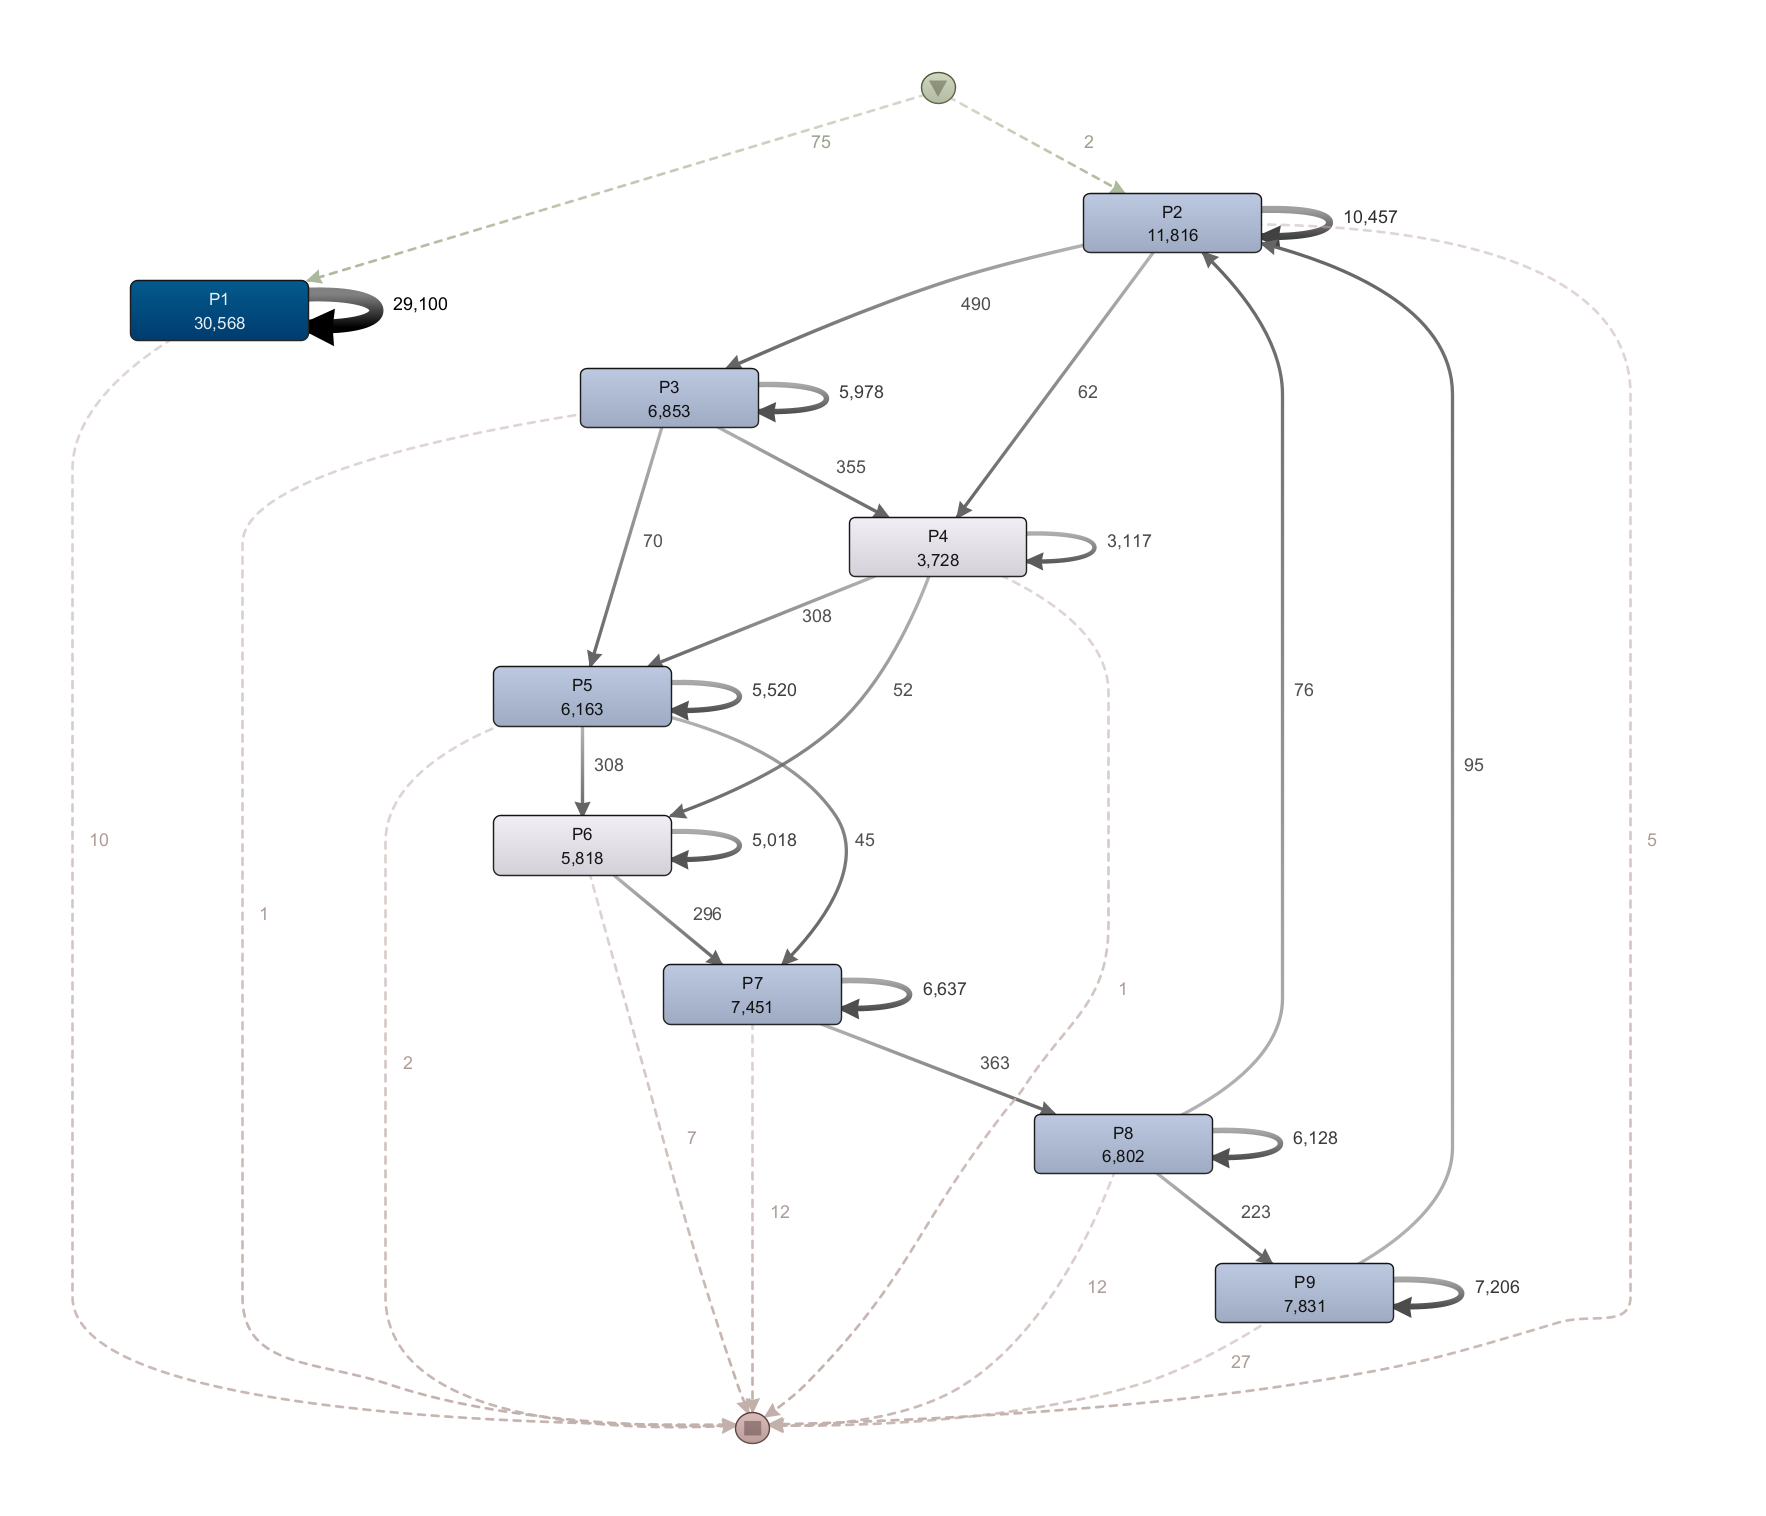
\includegraphics[width=\textwidth]{problems.png}
    \caption{Análisis de procesos del dataset (\texttt{Activity} problema y \texttt{CaseId} grupo). Contiene el $100\%$ de las actividades y el $80\%$ de los caminos.}
    \label{fig:problems}
\end{figure}

\begin{figure}[H]
    \centering
    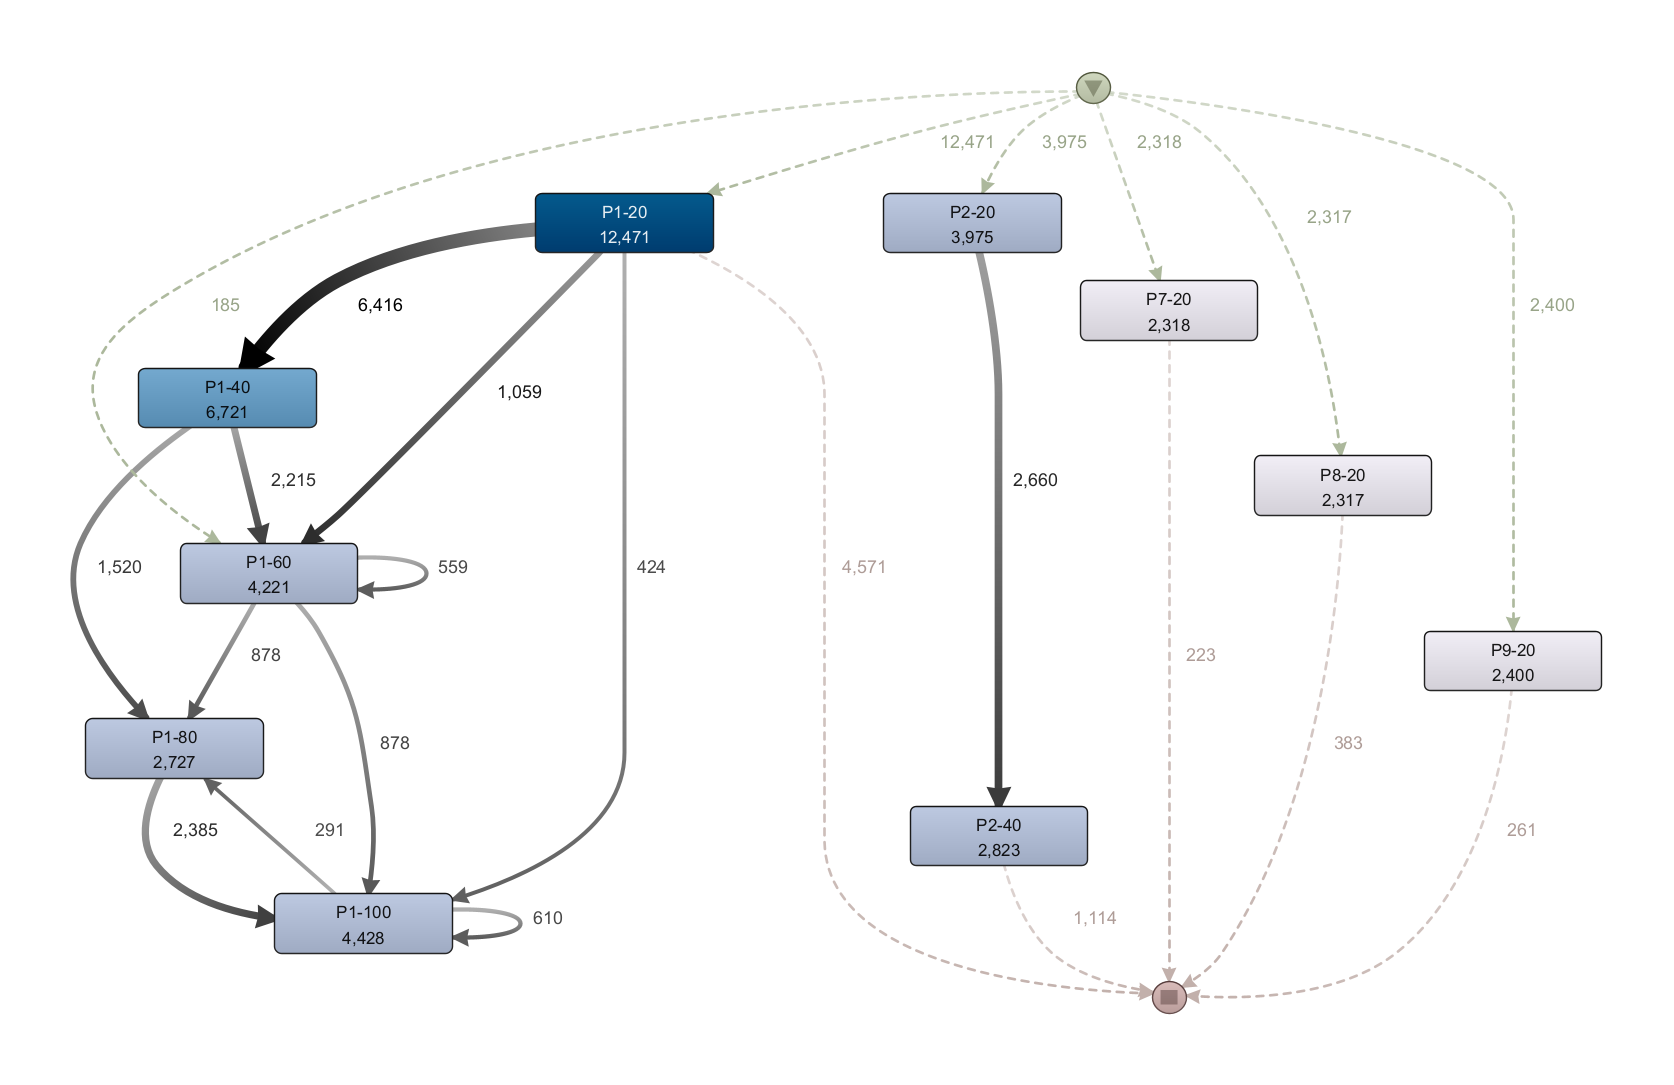
\includegraphics[width=\textwidth]{compound.png}
    \caption{Análisis de procesos del dataset (\texttt{Activity} problema-milestone y \texttt{CaseId} sesión). Contiene el $20\%$ de las actividades y el $20\%$ de los caminos.}
    \label{fig:compound}
\end{figure}

No obstante, a pesar de que tener una visión global del comportamiento de todos los grupos puede ayudar, nuestro objetivo final es poder caracterizar los comportamientos de los grupos y poder discernir, usando los datos del diagrama, si. Es por esto que nos será más interesante segmentar por grupos. Así pues, filtrando por el grupo \texttt{DBA 1516 P2 GA}, obtenemos los diagramas de las Figuras \ref{fig:problemsDBA1516P2GA} y \ref{fig:compoundDBA1516P2GA}.

\begin{figure}[H]
    \centering
    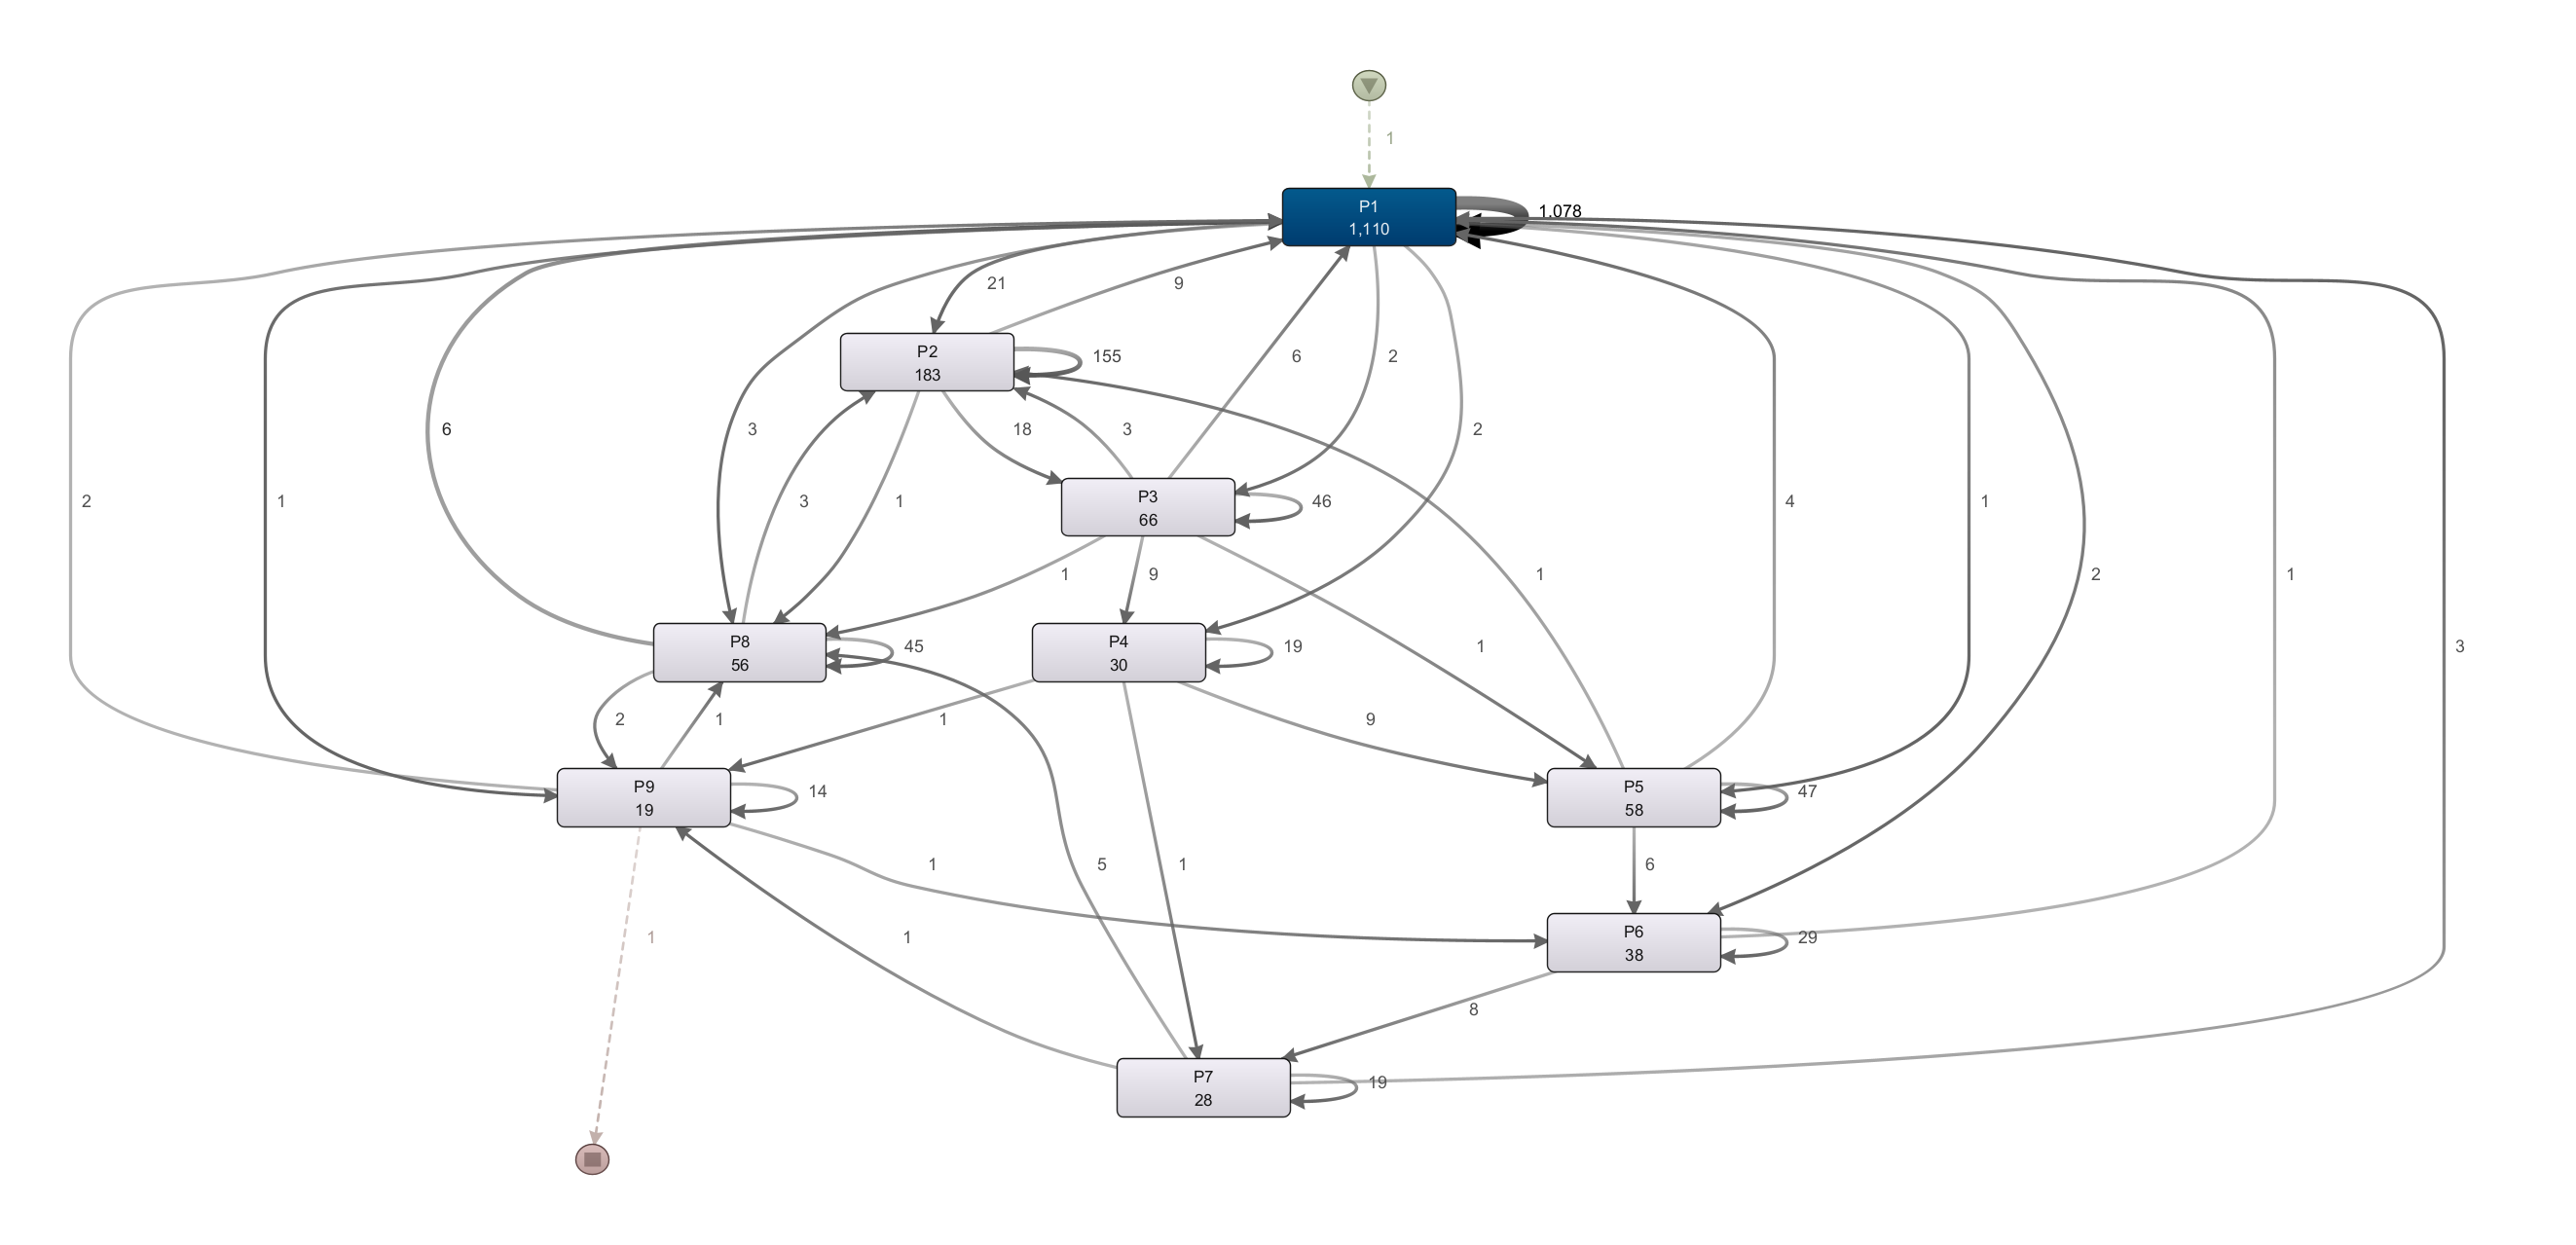
\includegraphics[width=\textwidth]{DBA1516P2GAProblems.png}
    \caption{Análisis de procesos del grupo \texttt{DBA 1516 P2 GA} (\texttt{Activity} problema y \texttt{CaseId} grupo). Contiene el $100\%$ de las actividades y el $100\%$ de los caminos.}
    \label{fig:problemsDBA1516P2GA}
\end{figure}

\begin{figure}[H]
    \centering
    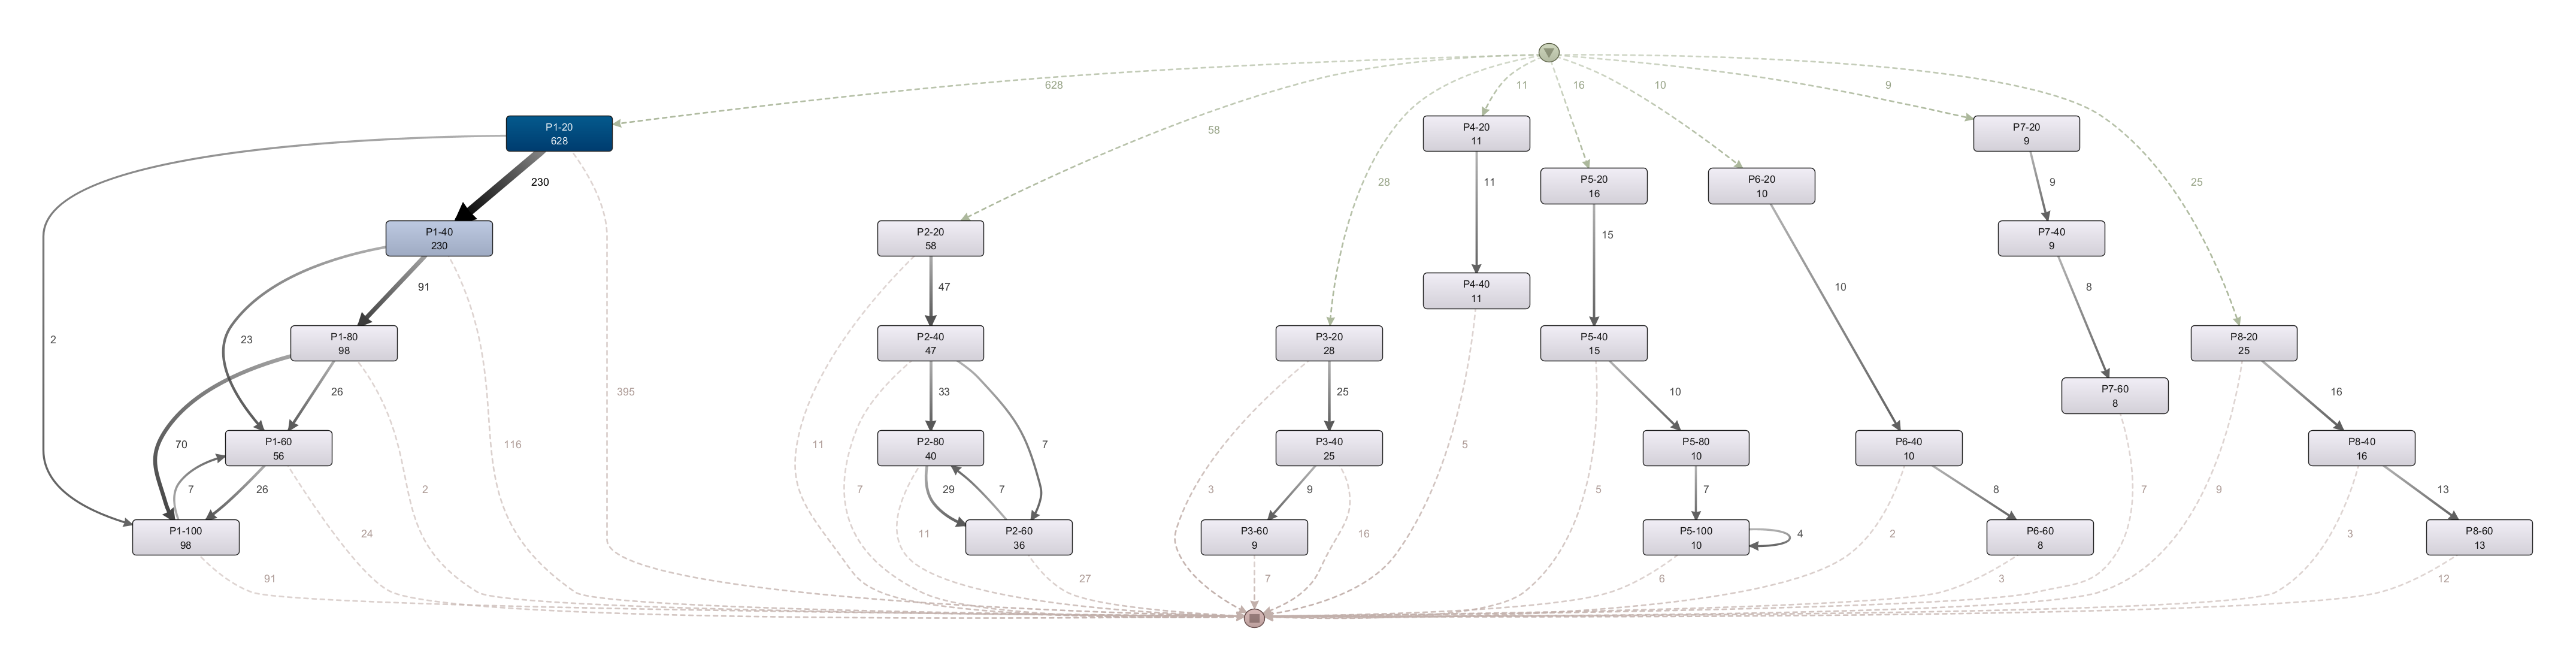
\includegraphics[width=\textwidth]{DBA1516P2GACompound.png}
    \caption{Análisis de procesos del grupo \texttt{DBA 1516 P2 GA} (\texttt{Activity} problema-milestone y \texttt{CaseId} sesión). Contiene el $60\%$ de las actividades y el $80\%$ de los caminos.}
    \label{fig:compoundDBA1516P2GA}
\end{figure}

Sin embargo, tras una larga experimentación con el programa Disco, se empiezan a ver sus limitaciones. En primer lugar, aunque Disco permite el filtrado de datos, si se quiere segmentar por grupos y extraer los procesos ocultos de cada uno de los grupos, hay que seleccionar el correspondiente grupo en el filtro, extraer los diagramas correspondientes e ir cambiandolo manualmente. Dado que tenemos un total de $77$ grupos de alumnos en los siete cursos académicos que forman parte del estudio (que pueden consultarse en las Tablas \ref{tab:groups1} y \ref{tab:groups2}), es inviable seguir usando el programa.

Así pues, en este trabajo fin de grado se ha implementado nuestra propia versión del programa, personalizada y adaptada a las necesidades del problema.